% Boundary Layer Illustration for Chattering Reduction
% TikZ diagram for Chapter 3 - Classical SMC

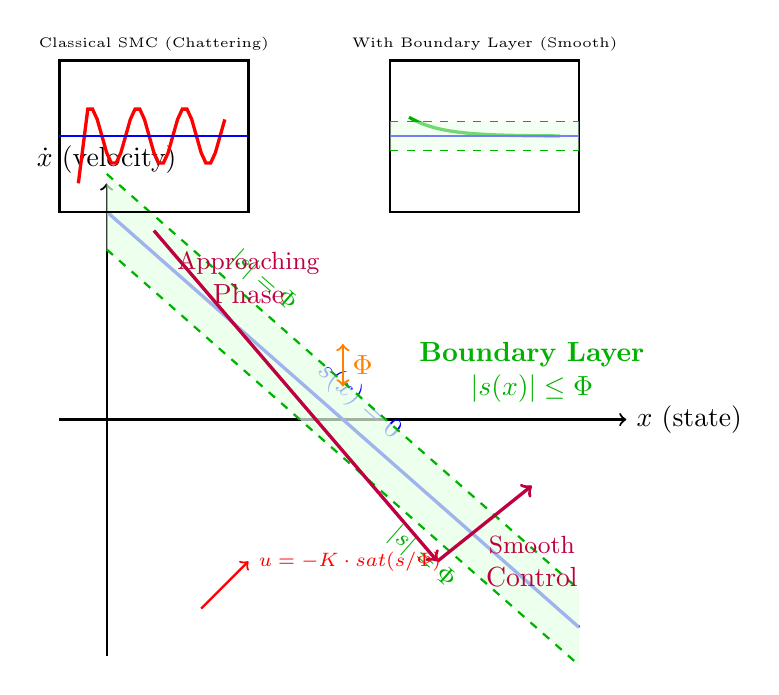
\begin{tikzpicture}[scale=1.2]

    % Axes
    \draw[->, thick] (-0.5, 0) -- (5.5, 0) node[right] {$x$ (state)};
    \draw[->, thick] (0, -2.5) -- (0, 2.5) node[above] {$\dot{x}$ (velocity)};

    % Sliding line
    \draw[blue, very thick] (0, 2.2) -- (5, -2.2)
        node[pos=0.5, above, sloped] {$s(\vect{x}) = 0$};

    % Boundary layer (shaded region around sliding line)
    \fill[green!10, opacity=0.7]
        (0, 2.6) -- (5, -1.8) -- (5, -2.6) -- (0, 1.8) -- cycle;

    % Boundary layer boundaries
    \draw[green!70!black, thick, dashed] (0, 2.6) -- (5, -1.8)
        node[pos=0.3, above, sloped, font=\small] {$|s| = \Phi$};
    \draw[green!70!black, thick, dashed] (0, 1.8) -- (5, -2.6)
        node[pos=0.7, below, sloped, font=\small] {$|s| = \Phi$};

    % Label boundary layer
    \node[green!70!black, align=center] at (4.5, 0.5) {
        \textbf{Boundary Layer}\\$|s(\vect{x})| \leq \Phi$
    };

    % Trajectory with chattering (without boundary layer)
    \begin{scope}[xshift=-0.5cm, yshift=3cm]
        % Zoomed inset showing chattering
        \draw[thick] (0, -0.8) rectangle (2, 0.8);
        \node[above] at (1, 0.8) {\tiny Classical SMC (Chattering)};

        % Chattering trajectory
        \draw[red, very thick] (0.2, -0.5)
            \foreach \x in {0.3, 0.35, ..., 1.8} {
                -- (\x, {0.3*sin((\x-0.2)*720)})
            };

        % Sliding line in inset
        \draw[blue, thick] (0, 0) -- (2, 0);
    \end{scope}

    % Trajectory with boundary layer (smooth)
    \begin{scope}[xshift=3cm, yshift=3cm]
        % Zoomed inset showing smooth behavior
        \draw[thick] (0, -0.8) rectangle (2, 0.8);
        \node[above] at (1, 0.8) {\tiny With Boundary Layer (Smooth)};

        % Smooth trajectory
        \draw[green!70!black, very thick, samples=50, smooth, domain=0.2:1.8]
            plot (\x, {0.2*exp(-3*(\x-0.2))});

        % Sliding line in inset
        \draw[blue, thick] (0, 0) -- (2, 0);

        % Boundary layer in inset
        \fill[green!10, opacity=0.5] (0, 0.15) rectangle (2, -0.15);
        \draw[green!70!black, dashed] (0, 0.15) -- (2, 0.15);
        \draw[green!70!black, dashed] (0, -0.15) -- (2, -0.15);
    \end{scope}

    % Main trajectory entering boundary layer
    \draw[->, very thick, purple, samples=40, smooth, domain=0:1]
        plot ({0.5 + 3*\x}, {2 - 3.5*\x});

    % Smooth continuation inside boundary layer
    \draw[->, very thick, purple, samples=50, smooth, domain=0:1]
        plot ({3.5 + 1*\x}, {-1.5 + 0.8*\x});

    % Annotations
    \node[purple, align=center] at (1.5, 1.5) {
        \small Approaching\\Phase
    };

    \node[purple, align=center] at (4.5, -1.5) {
        \small Smooth\\Control
    };

    % Boundary layer thickness annotation
    \draw[<->, thick, orange] (2.5, 0.8) -- (2.5, 0.35);
    \node[orange, right] at (2.5, 0.575) {$\Phi$};

    % Saturation function illustration
    \draw[->, thick, red] (1, -2) -- (1.5, -1.5)
        node[right, align=left] {\scriptsize $u = -K \cdot \text{sat}(s/\Phi)$};

\end{tikzpicture}
